\newcommand{\CourseTemplatePath}{../../../../../templates/slides/}
\input{\CourseTemplatePath course_preamble.tex}
\newcommand{\E}{\mathbb E}
\newcommand{\Sset}{\mathcal S}
\newcommand{\Aset}{\mathcal A}
\title[Simulation-Based Learning]{Lecture: Simulation-Based Learning}
\begin{document}
\makecoursetitle

\begin{frame}{Lecture Overview}
\small
\begin{itemize}
\item \textbf{From expected updates to sampled targets}
\begin{itemize}\item What an update aims at, and how simulation supplies its inputs\end{itemize}
\item \textbf{Two targets: Monte Carlo and TD(0)}
\begin{itemize}\item Complete returns versus bootstrapped targets: derivations and worked updates\end{itemize}
\item \textbf{Comparing targets and learning reliably}
\begin{itemize}\item Practical lessons on step sizes, visits, and accuracy\end{itemize}
\item \textbf{Optional extension}
\begin{itemize}\item Multi-step returns and TD(\(\lambda\))\end{itemize}
\end{itemize}
\end{frame}

\begin{frame}{From the Bellman Equation to Sampled Targets}
\small
\[
V^\sigma(s)=\underbrace{r(s,\sigma(s))+\beta\,
\tikz[baseline=(expect.base)]{
\node[draw=SessionTeal,circle,inner sep=1.3pt] (expect) {$\E$};
\node[overlay,above=8pt,font=\scriptsize] at (expect.north) {average over all possible next states};
\draw[SessionTeal] (expect.north)--++(0,.22);
\path (0,.75);
}
[V^\sigma(s')\mid s,a=\sigma(s)]}_{\text{Bellman target}}.
\]
Replacing \(\modelvar{V^\sigma}\) on the right by the current \(\modelvar{V}\) gives the \term{update target} \(\modelvar{T_\sigma V}\).
\begin{itemize}
\item \textbf{Continuous-state example:} For continuous future productivity, integrate over its conditional distribution.
\item Simulation replaces costly integration with sampled transitions and rewards.
\end{itemize}
\smallskip
\textbf{Can realized experience supply an update target?}
\par\medskip
We will follow one maze episode through two methods: \term{Monte Carlo (MC)} and \term{temporal-difference (TD)} learning.
\par\medskip
First observe the experience; then decide what target to construct from it.
\end{frame}

\begin{frame}{One Maze Episode, Two Ways to Learn}
\begin{columns}[c,onlytextwidth]
\begin{column}{.45\textwidth}
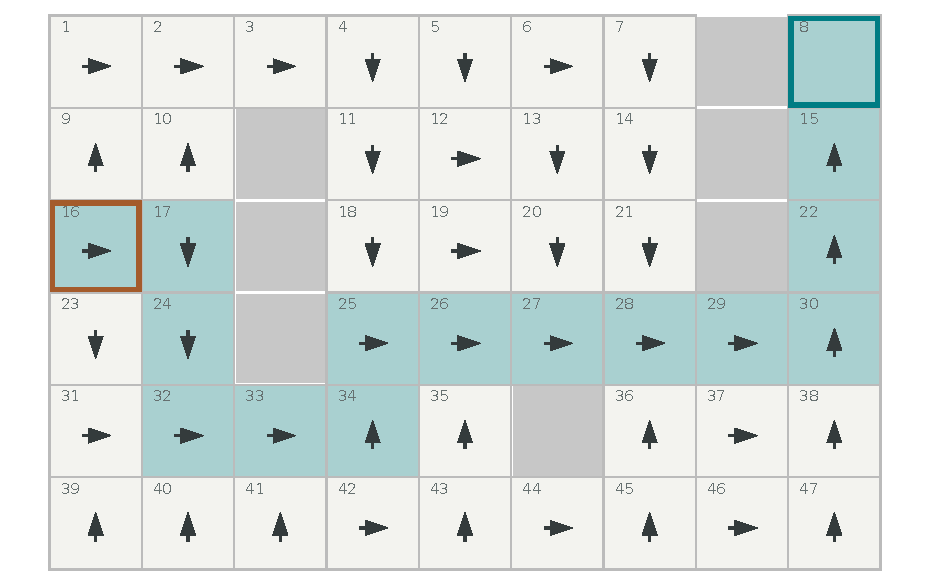
\includegraphics[width=\linewidth]{figures/simulation_coverage.pdf}
\par\smallskip\scriptsize Arrows: policy actions. Orange outline: usual start; teal outline: goal. Teal cells lie on the route from cell 16.
\end{column}
\begin{column}{.52\textwidth}\small
\courseexample{Random delays:} An action succeeds with probability \(\modelvar{.9}\); otherwise the agent stays in place.
\par\medskip
\textbf{Observed episode:} Start at cell 22 and take up at every step.
\begin{center}\begin{tabular}{clc}\toprule
Time & Transition & Reward\\\midrule
0 & \(22\to22\) (delay) & \(-1\)\\
1 & \(22\to15\) & \(-1\)\\
2 & \(15\to8\) (terminal) & \(-1\)\\\bottomrule
\end{tabular}\end{center}
\textbf{Comparison convention:} Both methods use the same policy and estimate the same \(\modelvar{V^\sigma}\).
\end{column}\end{columns}
\medskip
\small A \term{trajectory} is a sequence of states, actions, and rewards. An \term{episode} is a complete trajectory from a starting state to termination (here, the goal).
\end{frame}



\begin{frame}{MC: Wait for the Complete Return}
\small
The \term{complete discounted return}, for terminal time \(\modelvar{T}\), is
\[G_t=\sum_{j=0}^{T-t-1}\beta^j r_{t+j+1},\qquad V^\sigma(s)=\E_\sigma[G_t\mid s_t=s].\]
\courseexample{The same maze episode}
\[s_0:\text{ cell 22}\xrightarrow{r_1=-1}s_1:\text{ cell 22}
\xrightarrow{r_2=-1}s_2:\text{ cell 15}
\xrightarrow{r_3=-1}s_3=s_T:\text{ cell 8}\quad (T=3).\]
After termination, work backward from the final reward:
\[\begin{aligned}
G_2&=r_3=-1,\\
G_1&=r_2+\beta G_2=-1+.9(-1)=-1.9,\\
G_0&=r_1+\beta G_1=-1+.9(-1.9)=-2.71.
\end{aligned}\]
\term{First visit} means the first time a state appears within an episode. Cell 22 appears at \(\modelvar{t=0}\) and \(\modelvar{t=1}\): use \(\modelvar{G_0=-2.71}\) once. For cell 15, use \(\modelvar{G_2=-1}\).
\end{frame}

\begin{frame}{From Sample Returns to an Incremental Estimate}
\small
For \(\modelvar{n}\) independent first-visit returns at \(\modelvar{s}\), split off the last return:
\[V_n(s)=\frac1n\sum_{j=1}^{n}G^{[j]}(s)
=\frac{n-1}{n}V_{n-1}(s)+\frac1nG^{[n]}(s).\]
Rearranging gives the recursive update:
\[V_n(s)=V_{n-1}(s)+\frac1n\bigl[G^{[n]}(s)-V_{n-1}(s)\bigr].\]
With \(\modelvar{V_1(s)=G^{[1]}(s)}\), induction verifies the sample-mean formula for every \(\modelvar{n}\).
\par
\courseexample{Two episodes starting at cell 22}
\begin{itemize}
\item Previous trajectory: \(\modelvar{22\to22\to15\to8}\). Return \(\modelvar{-2.71}\); first estimate \(\modelvar{V_1(22)=-2.71}\).
\item Next trajectory: \(\modelvar{22\to15\to8}\). Return \(\modelvar{-1.9}\); new mean \(\modelvar{V_2(22)=-2.305}\).
\end{itemize}

\begin{itemize}
\item Complete returns are unbiased targets; averaging reduces sampling error.
\item Each target becomes available after its episode terminates.
\end{itemize}
\end{frame}

\begin{frame}{First-Visit MC: Policy Evaluation Algorithm}
\small
\begin{enumerate}
\setcounter{enumi}{-1}
\item \textbf{Inputs.} Fixed policy \(\modelvar{\sigma}\), discount \(\modelvar{\beta}\), starting-state distribution \(\modelvar{\mu_0}\), and episode budget \(\modelvar{K}\). Episodes terminate with finite expected length.
\item \textbf{Initialize.} Set \(\modelvar{V(s)=0}\) and \(\modelvar{N(s)=0}\) for every state; keep terminal values zero.
\item \textbf{Generate an episode.} Draw \(\modelvar{s_0\sim\mu_0}\), follow \(\modelvar{\sigma}\), and record states and rewards until termination.
\item \textbf{Compute returns backward.} Set \(\modelvar{G_T=0}\), then
\[G_t=r_{t+1}+\beta G_{t+1},\qquad t=T-1,\ldots,0.\]
\item \textbf{Update each first-visited state once.} At its earliest occurrence \(\modelvar{t}\), set
\[N(s_t)\leftarrow N(s_t)+1,\qquad
V(s_t)\leftarrow V(s_t)+\frac{G_t-V(s_t)}{N(s_t)}.\]
\item \textbf{Repeat and return.} Repeat Steps 2--4 for \(\modelvar{K}\) episodes. Return \(\modelvar{V}\) and the visit counts \(\modelvar{N}\).
\end{enumerate}
\end{frame}

\begin{frame}{TD: Update Before the Episode Ends}
\small
MC waits for the complete return. TD replaces the unobserved remaining return with the current continuation estimate:
\[
\underbrace{G_t=r_{t+1}+\beta G_{t+1}}_{\text{MC: wait for future rewards}}
\qquad\longrightarrow\qquad
\underbrace{r_{t+1}+\beta V_t(s_{t+1})}_{\text{TD target: available after one transition}}.
\]
\term{Bootstrapping} means using an estimated continuation value in the target.
\par\medskip
\courseexample{The first transition of the same episode}
\[s_0:\text{ cell 22}\xrightarrow{r_1=-1}s_1:\text{ cell 22}\qquad\text{future rewards not yet observed}\]
\[r_1+\beta V_0(s_1)=-1+.9V_0(22).\]
Averaging this target over possible next transitions recovers the expected DP update:
\[\E[r_{t+1}+\beta V_t(s_{t+1})\mid s_t=s,V_t]=(T_\sigma V_t)(s).\]
\end{frame}

\begin{frame}{TD(0): Move Toward the TD Target}
\small
\[\delta_t=\underbrace{r_{t+1}+\beta V_t(s_{t+1})}_{\text{TD target}}-V_t(s_t),\qquad
V_{t+1}(s_t)=V_t(s_t)+\alpha_n(s_t)\delta_t.\]
The \term{TD error} is target minus estimate; \(\modelvar{n}\) counts updates at \(\modelvar{s_t}\).
\par\smallskip
\courseexample{The same episode; initialize \(\modelvar{V_0=0}\), use \(\modelvar{\alpha_n(s)=.5}\)}
\[s_0:\text{ cell 22}\xrightarrow{r_1=-1}s_1:\text{ cell 22}
\xrightarrow{r_2=-1}s_2:\text{ cell 15}\xrightarrow{r_3=-1}s_3=s_T:\text{ cell 8}.\]
\begin{center}\renewcommand{\arraystretch}{1.2}\begin{tabular}{cll}\toprule
\(t\) & TD target: symbols, then numbers & Updated value\\\midrule
0 & \(r_1+\beta V_0(s_1)=-1+.9(0)=-1\) & \(V_1(22)=0+.5(-1)=-.5\)\\
1 & \(r_2+\beta V_1(s_2)=-1+.9(0)=-1\) & \(V_2(22)=-.5+.5(-.5)=-.75\)\\
2 & \(r_3+\beta V_2(s_3)=-1+.9(0)=-1\) & \(V_3(15)=0+.5(-1)=-.5\)\\\bottomrule
\end{tabular}\end{center}
Only the current state is updated; all other estimates retain their previous values.
\end{frame}

\begin{frame}{TD(0) Policy Evaluation: Algorithm}
\small
\begin{enumerate}
\setcounter{enumi}{-1}
\item \textbf{Inputs.} Fixed policy \(\modelvar{\sigma}\), discount \(\modelvar{\beta}\), starting distribution \(\modelvar{\mu_0}\), step budget \(\modelvar{B}\), and state-visit step sizes \(\modelvar{\alpha_n(s)}\).
\item \textbf{Initialize.} Set \(\modelvar{V=0}\), \(\modelvar{N=0}\), and draw \(\modelvar{s\sim\mu_0}\). Keep terminal values zero.
\item \textbf{Observe one transition.} Take \(\modelvar{a=\sigma(s)}\), receive \(\modelvar{r=r(s,a)}\), and observe \(\modelvar{s'}\).
\item \textbf{Update one state.} Increment \(\modelvar{N(s)}\), set \(\modelvar{n=N(s)}\), and compute the TD target before changing \(\modelvar{V(s)}\):
\[V(s)\leftarrow V(s)+\alpha_n(s)\,[r+\beta V(s')-V(s)].\]
\item \textbf{Advance or restart.} Set \(\modelvar{s=s'}\). If terminal, start a new episode from \(\modelvar{\mu_0}\).
\item \textbf{Repeat and return.} Repeat Steps 2--4 for \(\modelvar{B}\) transitions. Return \(\modelvar{V}\) and \(\modelvar{N}\).
\end{enumerate}
\end{frame}

\begin{frame}{Different Targets, the Same Objective}
\small
\textbf{Objective:} Estimate the value of each state under the same policy.
\par\medskip
\renewcommand{\arraystretch}{1.6}
\begin{tabular}{@{}>{\raggedright\arraybackslash}p{.15\textwidth}>{\raggedright\arraybackslash}p{.40\textwidth}>{\raggedright\arraybackslash}p{.36\textwidth}@{}}
\toprule
Method & What the target uses & When it is available\\\midrule
DP & An expectation calculated from the model & After model calculation\\
MC & A complete realized return & After the episode\\
TD & One reward plus estimated continuation & After one transition\\\bottomrule
\end{tabular}
\par\bigskip
\textbf{What makes sampled updates useful?} How much each update changes the estimate, which states receive updates, and how accuracy is checked.
\end{frame}

\begin{frame}{TD Step Size Controls the Size of Each Update}
\centering
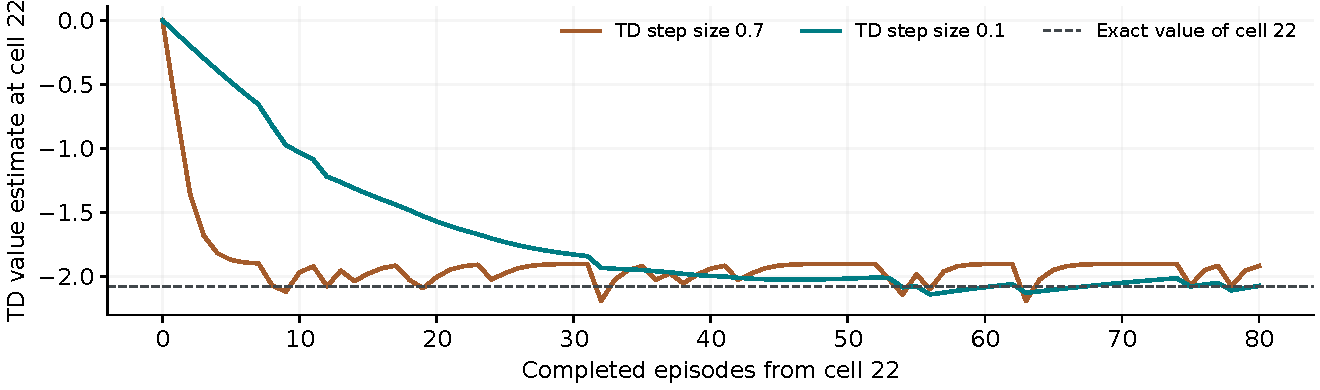
\includegraphics[height=4.2cm]{figures/simulation_step_sizes.pdf}
\par\smallskip\footnotesize Same policy and observed transitions; both TD runs start from zero.
\par\medskip\raggedright\small
\begin{itemize}
\item Large TD steps react quickly to new transitions but fluctuate more.
\item Small TD steps change estimates more slowly and smooth the fluctuations.
\end{itemize}
\end{frame}

\begin{frame}{Starting States Determine Which Values Can Be Learned}
\centering
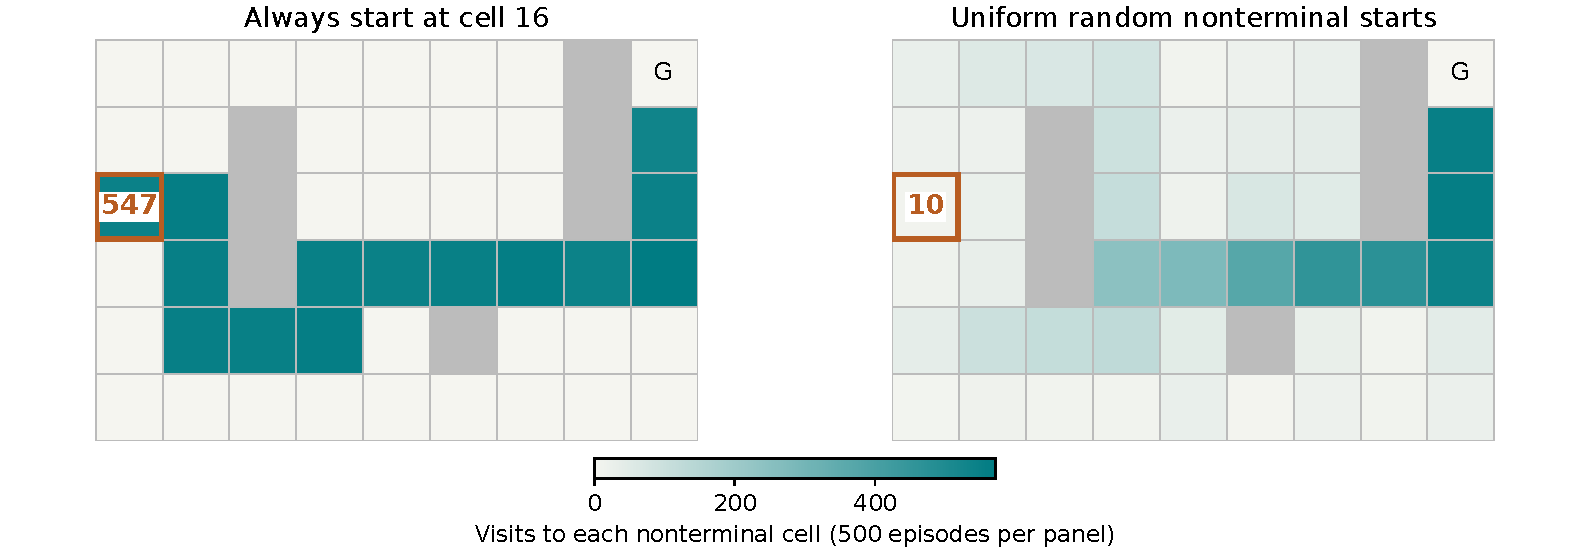
\includegraphics[height=3.5cm]{figures/simulation_visit_counts.pdf}
\par\smallskip
\raggedright\footnotesize
\textbf{Colors:} Darker teal = more visits; white = no visits; gray = wall; G = goal.
\par\smallskip
\textbf{Orange cell 16:} 547 visits with fixed starts; 10 with random starts, over 500 episodes in each panel. Repeat visits during delays count again, so visits can exceed episodes.
\par\medskip\raggedright\small
\begin{itemize}
\item Fixed starts leave 32 nonterminal cells without updates.
\item Random starts reach all 46 nonterminal cells, so we use them in the comparison.
\end{itemize}
\end{frame}

\begin{frame}{Measuring Accuracy against Exact DP}
\small
\textbf{For this small maze, exact DP gives a benchmark.}
\begin{enumerate}
\item \textbf{Compute the reference values.} Solve the fixed-policy Bellman equations using the known model.
\item \textbf{Give MC and TD the same experience.} Use the same policy and episodes, with random starting cells. MC averages returns; TD uses decreasing step sizes.
\item \textbf{Compare estimates with the reference.} Summarize their differences across all 46 nonterminal cells using root mean squared error (RMSE). Smaller means closer to the exact values.
\end{enumerate}
\end{frame}



\begin{frame}{MC and TD Accuracy in the Maze}
\centering
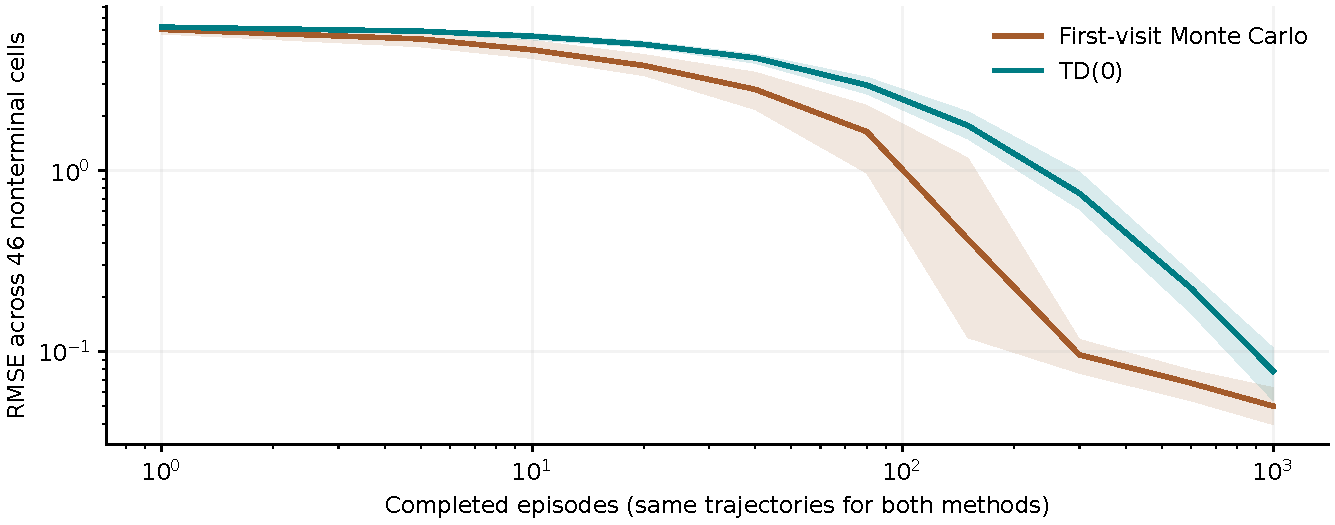
\includegraphics[height=3.6cm]{figures/simulation_mc_td.pdf}
\par\smallskip\raggedright\footnotesize
\textbf{Horizontal:} completed episodes (experience). \textbf{Vertical:} error against exact DP (lower is better). Lines average 20 runs; bands show variation across runs.
\par\smallskip\small
\begin{itemize}
\item Both methods improve with experience; MC has lower error here.
\item MC gets complete returns throughout the maze; TD must learn continuation values. Starting states and step sizes also affect the comparison.
\item Chapter 6's random walk favors TD: this result is specific to the task and learning settings.
\end{itemize}
\end{frame}







\begin{frame}{Optional: Between TD and Monte Carlo}
\small
We can wait for more rewards before using a continuation estimate.
\begin{itemize}
\item \textbf{After one transition:} the TD(0) target
\[r_{t+1}+\beta V_t(s_{t+1}).\]
\item \textbf{After two transitions:} use two rewards and the current estimate
\[r_{t+1}+\beta r_{t+2}+\beta^2 V_{t+1}(s_{t+2}).\]
\item \textbf{At termination:} use the complete return \(\modelvar{G_t}\), with no continuation estimate.
\end{itemize}
\medskip
If the episode ends earlier, stop at termination and use the remaining realized rewards.
\par\medskip
\term{TD(\(\lambda\))} combines targets with different waiting lengths. It connects one-step TD with learning from longer returns.
\end{frame}

% BEGIN MANAGED READINGS: week5_simulation
\begin{frame}{References and Further Reading}
\coursereading{1}
  {Richard S. Sutton and Andrew G. Barto (2018), Reinforcement Learning: An Introduction. 2nd ed. MIT Press. [Book]}
  {https://www.andrew.cmu.edu/course/10-703/textbook/BartoSutton.pdf}
  {\begin{itemize}
\item \href{https://www.andrew.cmu.edu/course/10-703/textbook/BartoSutton.pdf\#page=113}{Chapter 5: Monte Carlo Methods}
\item \href{https://www.andrew.cmu.edu/course/10-703/textbook/BartoSutton.pdf\#page=141}{Chapter 6: Temporal-Difference Learning}
\item \href{https://www.andrew.cmu.edu/course/10-703/textbook/BartoSutton.pdf\#page=163}{Chapter 7: n-step Bootstrapping (optional)}
\item \href{https://www.andrew.cmu.edu/course/10-703/textbook/BartoSutton.pdf\#page=309}{Chapter 12: Eligibility Traces (optional)}
\end{itemize}}
\end{frame}
% END MANAGED READINGS: week5_simulation
\end{document}
